\documentclass[twoside]{book}

% Packages required by doxygen
\usepackage{fixltx2e}
\usepackage{calc}
\usepackage{doxygen}
\usepackage[export]{adjustbox} % also loads graphicx
\usepackage{graphicx}
\usepackage[utf8]{inputenc}
\usepackage{makeidx}
\usepackage{multicol}
\usepackage{multirow}
\PassOptionsToPackage{warn}{textcomp}
\usepackage{textcomp}
\usepackage[nointegrals]{wasysym}
\usepackage[table]{xcolor}

% Font selection
\usepackage[T1]{fontenc}
\usepackage[scaled=.90]{helvet}
\usepackage{courier}
\usepackage{amssymb}
\usepackage{sectsty}
\renewcommand{\familydefault}{\sfdefault}
\allsectionsfont{%
  \fontseries{bc}\selectfont%
  \color{darkgray}%
}
\renewcommand{\DoxyLabelFont}{%
  \fontseries{bc}\selectfont%
  \color{darkgray}%
}
\newcommand{\+}{\discretionary{\mbox{\scriptsize$\hookleftarrow$}}{}{}}

% Page & text layout
\usepackage{geometry}
\geometry{%
  a4paper,%
  top=2.5cm,%
  bottom=2.5cm,%
  left=2.5cm,%
  right=2.5cm%
}
\tolerance=750
\hfuzz=15pt
\hbadness=750
\setlength{\emergencystretch}{15pt}
\setlength{\parindent}{0cm}
\setlength{\parskip}{3ex plus 2ex minus 2ex}
\makeatletter
\renewcommand{\paragraph}{%
  \@startsection{paragraph}{4}{0ex}{-1.0ex}{1.0ex}{%
    \normalfont\normalsize\bfseries\SS@parafont%
  }%
}
\renewcommand{\subparagraph}{%
  \@startsection{subparagraph}{5}{0ex}{-1.0ex}{1.0ex}{%
    \normalfont\normalsize\bfseries\SS@subparafont%
  }%
}
\makeatother

% Headers & footers
\usepackage{fancyhdr}
\pagestyle{fancyplain}
\fancyhead[LE]{\fancyplain{}{\bfseries\thepage}}
\fancyhead[CE]{\fancyplain{}{}}
\fancyhead[RE]{\fancyplain{}{\bfseries\leftmark}}
\fancyhead[LO]{\fancyplain{}{\bfseries\rightmark}}
\fancyhead[CO]{\fancyplain{}{}}
\fancyhead[RO]{\fancyplain{}{\bfseries\thepage}}
\fancyfoot[LE]{\fancyplain{}{}}
\fancyfoot[CE]{\fancyplain{}{}}
\fancyfoot[RE]{\fancyplain{}{\bfseries\scriptsize Generated by Doxygen }}
\fancyfoot[LO]{\fancyplain{}{\bfseries\scriptsize Generated by Doxygen }}
\fancyfoot[CO]{\fancyplain{}{}}
\fancyfoot[RO]{\fancyplain{}{}}
\renewcommand{\footrulewidth}{0.4pt}
\renewcommand{\chaptermark}[1]{%
  \markboth{#1}{}%
}
\renewcommand{\sectionmark}[1]{%
  \markright{\thesection\ #1}%
}

% Indices & bibliography
\usepackage{natbib}
\usepackage[titles]{tocloft}
\setcounter{tocdepth}{3}
\setcounter{secnumdepth}{5}
\makeindex

% Hyperlinks (required, but should be loaded last)
\usepackage{ifpdf}
\ifpdf
  \usepackage[pdftex,pagebackref=true]{hyperref}
\else
  \usepackage[ps2pdf,pagebackref=true]{hyperref}
\fi
\hypersetup{%
  colorlinks=true,%
  linkcolor=blue,%
  citecolor=blue,%
  unicode%
}

% Custom commands
\newcommand{\clearemptydoublepage}{%
  \newpage{\pagestyle{empty}\cleardoublepage}%
}

\usepackage{caption}
\captionsetup{labelsep=space,justification=centering,font={bf},singlelinecheck=off,skip=4pt,position=top}

%===== C O N T E N T S =====

\begin{document}

% Titlepage & ToC
\hypersetup{pageanchor=false,
             bookmarksnumbered=true,
             pdfencoding=unicode
            }
\pagenumbering{alph}
\begin{titlepage}
\vspace*{7cm}
\begin{center}%
{\Large My Project }\\
\vspace*{1cm}
{\large Generated by Doxygen 1.8.12}\\
\end{center}
\end{titlepage}
\clearemptydoublepage
\pagenumbering{roman}
\tableofcontents
\clearemptydoublepage
\pagenumbering{arabic}
\hypersetup{pageanchor=true}

%--- Begin generated contents ---
\chapter{Hierarchical Index}
\section{Class Hierarchy}
This inheritance list is sorted roughly, but not completely, alphabetically\+:\begin{DoxyCompactList}
\item \contentsline{section}{Chord\+User}{\pageref{class_chord_user}}{}
\item Input\+Stream\begin{DoxyCompactList}
\item \contentsline{section}{File\+Stream}{\pageref{class_file_stream}}{}
\end{DoxyCompactList}
\item Runnable\begin{DoxyCompactList}
\item \contentsline{section}{Shutdown}{\pageref{class_shutdown}}{}
\end{DoxyCompactList}
\item Serializable\begin{DoxyCompactList}
\item \contentsline{section}{File\+Stream}{\pageref{class_file_stream}}{}
\end{DoxyCompactList}
\item Thread\begin{DoxyCompactList}
\item \contentsline{section}{Shutdown}{\pageref{class_shutdown}}{}
\end{DoxyCompactList}
\item Unicast\+Remote\+Object\begin{DoxyCompactList}
\item \contentsline{section}{Chord}{\pageref{class_chord}}{}
\end{DoxyCompactList}
\item Remote\begin{DoxyCompactList}
\item \contentsline{section}{Chord\+Message\+Interface}{\pageref{interface_chord_message_interface}}{}
\begin{DoxyCompactList}
\item \contentsline{section}{Chord}{\pageref{class_chord}}{}
\end{DoxyCompactList}
\item \contentsline{section}{Shutdown\+Interface}{\pageref{interface_shutdown_interface}}{}
\begin{DoxyCompactList}
\item \contentsline{section}{Chord}{\pageref{class_chord}}{}
\end{DoxyCompactList}
\end{DoxyCompactList}
\end{DoxyCompactList}

\chapter{Class Index}
\section{Class List}
Here are the classes, structs, unions and interfaces with brief descriptions\+:\begin{DoxyCompactList}
\item\contentsline{section}{\hyperlink{class_chat}{Chat} \\*It implements a distributed chat. It creates a ring and delivers messages using flooding }{\pageref{class_chat}}{}
\item\contentsline{section}{\hyperlink{class_chat_1_1_client}{Chat.\+Client} \\*It implements the client }{\pageref{class_chat_1_1_client}}{}
\item\contentsline{section}{\hyperlink{enum_chat_1_1enum___m_s_g}{Chat.\+enum\+\_\+\+M\+SG} \\*Enum Class to keep track of message Ids }{\pageref{enum_chat_1_1enum___m_s_g}}{}
\item\contentsline{section}{\hyperlink{class_chat_1_1_main_message}{Chat.\+Main\+Message} \\*This class implements a main message. It keeps all the information the user would like to send to its peers }{\pageref{class_chat_1_1_main_message}}{}
\item\contentsline{section}{\hyperlink{class_chat_1_1_peer}{Chat.\+Peer} \\*This class implements a peer. It keeps the information of our peer simulating a doubly-\/linkedlist }{\pageref{class_chat_1_1_peer}}{}
\item\contentsline{section}{\hyperlink{class_chat_1_1_server}{Chat.\+Server} \\*It implements the server }{\pageref{class_chat_1_1_server}}{}
\end{DoxyCompactList}

\chapter{File Index}
\section{File List}
Here is a list of all files with brief descriptions\+:\begin{DoxyCompactList}
\item\contentsline{section}{C\+E\+C\+S 327/\+C\+E\+C\+S-\/327/\+Assignment\+\_\+2/\hyperlink{_chat_8java}{Chat.\+java} }{\pageref{_chat_8java}}{}
\end{DoxyCompactList}

\chapter{Class Documentation}
\hypertarget{class_chord}{}\section{Chord Class Reference}
\label{class_chord}\index{Chord@{Chord}}
Inheritance diagram for Chord\+:\begin{figure}[H]
\begin{center}
\leavevmode
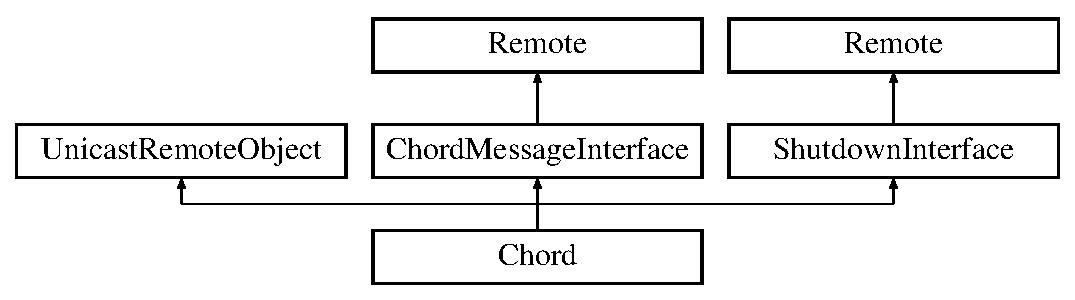
\includegraphics[height=3.000000cm]{class_chord}
\end{center}
\end{figure}
\subsection*{Public Member Functions}
\begin{DoxyCompactItemize}
\item 
\hyperlink{interface_chord_message_interface}{Chord\+Message\+Interface} \hyperlink{class_chord_a2fd46745a549fb8447f2cb7e32e8b07b}{rmi\+Chord} (String ip, int port)
\begin{DoxyCompactList}\small\item\em Makes the \hyperlink{interface_chord_message_interface}{Chord\+Message\+Interface} object accessable remotely. \end{DoxyCompactList}\item 
Boolean \hyperlink{class_chord_ad88edc3a01395c31dd0ae209195a2e08}{is\+Key\+In\+Semi\+Close\+Interval} (int key, int key1, int key2)
\begin{DoxyCompactList}\small\item\em Checks if the Key is in a Semi Close interval. \end{DoxyCompactList}\item 
Boolean \hyperlink{class_chord_a711a8c4e621940da4c48c1ba60479bd7}{is\+Key\+In\+Open\+Interval} (int key, int key1, int key2)
\begin{DoxyCompactList}\small\item\em Checks if the key is in Open Interval. \end{DoxyCompactList}\item 
void \hyperlink{class_chord_a88829ad2bea7d036256fd55dab5945fd}{put} (int guid, Input\+Stream file)  throws Remote\+Exception, File\+Not\+Found\+Exception, I\+O\+Exception 
\begin{DoxyCompactList}\small\item\em Gets the file and puts it in my repository. \end{DoxyCompactList}\item 
Input\+Stream \hyperlink{class_chord_a0425685114bc996226e87f417221c213}{get} (int guid)  throws Remote\+Exception, File\+Not\+Found\+Exception, I\+O\+Exception 
\begin{DoxyCompactList}\small\item\em Retrieves the file from my repository. \end{DoxyCompactList}\item 
void \hyperlink{class_chord_a83d9245c283baf440dc847cee154c8c6}{delete} (int guid)  throws Remote\+Exception 
\begin{DoxyCompactList}\small\item\em Deletes the file form my repository. \end{DoxyCompactList}\item 
int \hyperlink{class_chord_a7c6a50aff653bafc040f923c93061bdb}{get\+Id} ()  throws Remote\+Exception 
\item 
boolean \hyperlink{class_chord_a0a677ced19cc0cb5afd2a695977aeb95}{is\+Alive} ()  throws Remote\+Exception 
\begin{DoxyCompactList}\small\item\em Returns if I\textquotesingle{}m alive. \end{DoxyCompactList}\item 
\hyperlink{interface_chord_message_interface}{Chord\+Message\+Interface} \hyperlink{class_chord_a3f1aadce3820e808c80662bb61a58e34}{get\+Predecessor} ()  throws Remote\+Exception 
\begin{DoxyCompactList}\small\item\em Returns predecessor. \end{DoxyCompactList}\item 
\hyperlink{interface_chord_message_interface}{Chord\+Message\+Interface} \hyperlink{class_chord_aa53f4f7c97122395a33d064460538db0}{locate\+Successor} (int key)  throws Remote\+Exception 
\begin{DoxyCompactList}\small\item\em Locates successor. \end{DoxyCompactList}\item 
\hyperlink{interface_chord_message_interface}{Chord\+Message\+Interface} \hyperlink{class_chord_a77a9443c945cf5482f59edf685c1dc70}{closest\+Preceding\+Node} (int key)  throws Remote\+Exception 
\begin{DoxyCompactList}\small\item\em Locates closest Preceding Node. \end{DoxyCompactList}\item 
void \hyperlink{class_chord_ace0b8d2768590d7527af155c6573cae7}{join\+Ring} (String ip, int port)  throws Remote\+Exception 
\begin{DoxyCompactList}\small\item\em Joins the ring. \end{DoxyCompactList}\item 
void \hyperlink{class_chord_aa1906d1d721280b3a10a7754f604990a}{leave\+Ring} ()  throws Remote\+Exception     
\begin{DoxyCompactList}\small\item\em Leaves the ring. \end{DoxyCompactList}\item 
void \hyperlink{class_chord_a03cd68070e7cf5a96e015773df7ab034}{set\+Predeccesor} (\hyperlink{interface_chord_message_interface}{Chord\+Message\+Interface} m)
\begin{DoxyCompactList}\small\item\em Sets Predecessor. \end{DoxyCompactList}\item 
void \hyperlink{class_chord_a7de61846981d5fd1b7a9b8a6c653dc76}{set\+Successor} (\hyperlink{interface_chord_message_interface}{Chord\+Message\+Interface} m)
\begin{DoxyCompactList}\small\item\em Sets Successor. \end{DoxyCompactList}\item 
void \hyperlink{class_chord_a65c855dc1d8c6a82545899cb823dba2e}{finding\+Next\+Successor} ()
\begin{DoxyCompactList}\small\item\em Find Next Successor. \end{DoxyCompactList}\item 
void \hyperlink{class_chord_a8a4b7a1cd88cb3f607ada0629f2ff2dd}{stabilize} ()
\begin{DoxyCompactList}\small\item\em Stabilizes the successor and make sure that files in the repository are up to date. \end{DoxyCompactList}\item 
void \hyperlink{class_chord_a4de8b8464782dd96d88deeb35b2f27a2}{notify} (\hyperlink{interface_chord_message_interface}{Chord\+Message\+Interface} j)  throws Remote\+Exception 
\begin{DoxyCompactList}\small\item\em Notify checks if my predecessor is null or if its an open interval with j and i if it is true for either then it copies those files to j\textquotesingle{}s repository. \end{DoxyCompactList}\item 
void \hyperlink{class_chord_a02763f74bbd986baa7e6567bf9dc3c95}{fix\+Fingers} ()
\begin{DoxyCompactList}\small\item\em Fixes the fingers so that they are up to date. \end{DoxyCompactList}\item 
void \hyperlink{class_chord_a530b2ab58c9f4026dadf4293c38c4450}{check\+Predecessor} ()
\begin{DoxyCompactList}\small\item\em Check Predecessor is alive otherwise set it to null. \end{DoxyCompactList}\item 
\hyperlink{class_chord_aed079e86ebb63da4af055ca324a74274}{Chord} (int port)  throws Remote\+Exception 
\begin{DoxyCompactList}\small\item\em \hyperlink{class_chord}{Chord} Constructor. \end{DoxyCompactList}\item 
void \hyperlink{class_chord_a8616150947d5fa4095187325bc9f8a60}{shutdown} ()  throws Remote\+Exception 
\begin{DoxyCompactList}\small\item\em \hyperlink{class_shutdown}{Shutdown} Function for Control + C command. \end{DoxyCompactList}\end{DoxyCompactItemize}
\subsection*{Static Public Attributes}
\begin{DoxyCompactItemize}
\item 
static final int \hyperlink{class_chord_a864e0b4011dc157c78a06dd951c6d9ac}{M} = 2
\end{DoxyCompactItemize}
\subsection*{Private Attributes}
\begin{DoxyCompactItemize}
\item 
\hyperlink{class_shutdown}{Shutdown} \hyperlink{class_chord_a41961ec2d829d7a2c765fe7f8a23a64c}{shutdown}
\end{DoxyCompactItemize}


\subsection{Constructor \& Destructor Documentation}
\hypertarget{class_chord_aed079e86ebb63da4af055ca324a74274}{}\label{class_chord_aed079e86ebb63da4af055ca324a74274} 
\index{Chord@{Chord}!Chord@{Chord}}
\index{Chord@{Chord}!Chord@{Chord}}
\subsubsection{\texorpdfstring{Chord()}{Chord()}}
{\footnotesize\ttfamily Chord.\+Chord (\begin{DoxyParamCaption}\item[{int}]{port }\end{DoxyParamCaption}) throws Remote\+Exception}



\hyperlink{class_chord}{Chord} Constructor. 

create the registry and bind the name and object. 

\subsection{Member Function Documentation}
\hypertarget{class_chord_a530b2ab58c9f4026dadf4293c38c4450}{}\label{class_chord_a530b2ab58c9f4026dadf4293c38c4450} 
\index{Chord@{Chord}!check\+Predecessor@{check\+Predecessor}}
\index{check\+Predecessor@{check\+Predecessor}!Chord@{Chord}}
\subsubsection{\texorpdfstring{check\+Predecessor()}{checkPredecessor()}}
{\footnotesize\ttfamily void Chord.\+check\+Predecessor (\begin{DoxyParamCaption}{ }\end{DoxyParamCaption})}



Check Predecessor is alive otherwise set it to null. 

\hypertarget{class_chord_a77a9443c945cf5482f59edf685c1dc70}{}\label{class_chord_a77a9443c945cf5482f59edf685c1dc70} 
\index{Chord@{Chord}!closest\+Preceding\+Node@{closest\+Preceding\+Node}}
\index{closest\+Preceding\+Node@{closest\+Preceding\+Node}!Chord@{Chord}}
\subsubsection{\texorpdfstring{closest\+Preceding\+Node()}{closestPrecedingNode()}}
{\footnotesize\ttfamily \hyperlink{interface_chord_message_interface}{Chord\+Message\+Interface} Chord.\+closest\+Preceding\+Node (\begin{DoxyParamCaption}\item[{int}]{key }\end{DoxyParamCaption}) throws Remote\+Exception}



Locates closest Preceding Node. 



Implements \hyperlink{interface_chord_message_interface_a7f47e9d5144a2af6904135bc05dfe8fd}{Chord\+Message\+Interface}.

\hypertarget{class_chord_a83d9245c283baf440dc847cee154c8c6}{}\label{class_chord_a83d9245c283baf440dc847cee154c8c6} 
\index{Chord@{Chord}!delete@{delete}}
\index{delete@{delete}!Chord@{Chord}}
\subsubsection{\texorpdfstring{delete()}{delete()}}
{\footnotesize\ttfamily void Chord.\+delete (\begin{DoxyParamCaption}\item[{int}]{guid }\end{DoxyParamCaption}) throws Remote\+Exception}



Deletes the file form my repository. 



Implements \hyperlink{interface_chord_message_interface_ab4d46beae8cea347c827b5618ea16104}{Chord\+Message\+Interface}.

\hypertarget{class_chord_a65c855dc1d8c6a82545899cb823dba2e}{}\label{class_chord_a65c855dc1d8c6a82545899cb823dba2e} 
\index{Chord@{Chord}!finding\+Next\+Successor@{finding\+Next\+Successor}}
\index{finding\+Next\+Successor@{finding\+Next\+Successor}!Chord@{Chord}}
\subsubsection{\texorpdfstring{finding\+Next\+Successor()}{findingNextSuccessor()}}
{\footnotesize\ttfamily void Chord.\+finding\+Next\+Successor (\begin{DoxyParamCaption}{ }\end{DoxyParamCaption})}



Find Next Successor. 

\hypertarget{class_chord_a02763f74bbd986baa7e6567bf9dc3c95}{}\label{class_chord_a02763f74bbd986baa7e6567bf9dc3c95} 
\index{Chord@{Chord}!fix\+Fingers@{fix\+Fingers}}
\index{fix\+Fingers@{fix\+Fingers}!Chord@{Chord}}
\subsubsection{\texorpdfstring{fix\+Fingers()}{fixFingers()}}
{\footnotesize\ttfamily void Chord.\+fix\+Fingers (\begin{DoxyParamCaption}{ }\end{DoxyParamCaption})}



Fixes the fingers so that they are up to date. 

\hypertarget{class_chord_a0425685114bc996226e87f417221c213}{}\label{class_chord_a0425685114bc996226e87f417221c213} 
\index{Chord@{Chord}!get@{get}}
\index{get@{get}!Chord@{Chord}}
\subsubsection{\texorpdfstring{get()}{get()}}
{\footnotesize\ttfamily Input\+Stream Chord.\+get (\begin{DoxyParamCaption}\item[{int}]{guid }\end{DoxyParamCaption}) throws Remote\+Exception, File\+Not\+Found\+Exception, I\+O\+Exception}



Retrieves the file from my repository. 



Implements \hyperlink{interface_chord_message_interface_a4cdb461c48fe643f4fb5fa420d017eb3}{Chord\+Message\+Interface}.

\hypertarget{class_chord_a7c6a50aff653bafc040f923c93061bdb}{}\label{class_chord_a7c6a50aff653bafc040f923c93061bdb} 
\index{Chord@{Chord}!get\+Id@{get\+Id}}
\index{get\+Id@{get\+Id}!Chord@{Chord}}
\subsubsection{\texorpdfstring{get\+Id()}{getId()}}
{\footnotesize\ttfamily int Chord.\+get\+Id (\begin{DoxyParamCaption}{ }\end{DoxyParamCaption}) throws Remote\+Exception}

Returns my Id 

Implements \hyperlink{interface_chord_message_interface_acead95d9a7196f05b656462ab78138eb}{Chord\+Message\+Interface}.

\hypertarget{class_chord_a3f1aadce3820e808c80662bb61a58e34}{}\label{class_chord_a3f1aadce3820e808c80662bb61a58e34} 
\index{Chord@{Chord}!get\+Predecessor@{get\+Predecessor}}
\index{get\+Predecessor@{get\+Predecessor}!Chord@{Chord}}
\subsubsection{\texorpdfstring{get\+Predecessor()}{getPredecessor()}}
{\footnotesize\ttfamily \hyperlink{interface_chord_message_interface}{Chord\+Message\+Interface} Chord.\+get\+Predecessor (\begin{DoxyParamCaption}{ }\end{DoxyParamCaption}) throws Remote\+Exception}



Returns predecessor. 



Implements \hyperlink{interface_chord_message_interface_ab07c08ba6088ef880eaf4ebae8281c51}{Chord\+Message\+Interface}.

\hypertarget{class_chord_a0a677ced19cc0cb5afd2a695977aeb95}{}\label{class_chord_a0a677ced19cc0cb5afd2a695977aeb95} 
\index{Chord@{Chord}!is\+Alive@{is\+Alive}}
\index{is\+Alive@{is\+Alive}!Chord@{Chord}}
\subsubsection{\texorpdfstring{is\+Alive()}{isAlive()}}
{\footnotesize\ttfamily boolean Chord.\+is\+Alive (\begin{DoxyParamCaption}{ }\end{DoxyParamCaption}) throws Remote\+Exception}



Returns if I\textquotesingle{}m alive. 



Implements \hyperlink{interface_chord_message_interface_a8165b3fb53905e657c70b66223197561}{Chord\+Message\+Interface}.

\hypertarget{class_chord_a711a8c4e621940da4c48c1ba60479bd7}{}\label{class_chord_a711a8c4e621940da4c48c1ba60479bd7} 
\index{Chord@{Chord}!is\+Key\+In\+Open\+Interval@{is\+Key\+In\+Open\+Interval}}
\index{is\+Key\+In\+Open\+Interval@{is\+Key\+In\+Open\+Interval}!Chord@{Chord}}
\subsubsection{\texorpdfstring{is\+Key\+In\+Open\+Interval()}{isKeyInOpenInterval()}}
{\footnotesize\ttfamily Boolean Chord.\+is\+Key\+In\+Open\+Interval (\begin{DoxyParamCaption}\item[{int}]{key,  }\item[{int}]{key1,  }\item[{int}]{key2 }\end{DoxyParamCaption})}



Checks if the key is in Open Interval. 

\hypertarget{class_chord_ad88edc3a01395c31dd0ae209195a2e08}{}\label{class_chord_ad88edc3a01395c31dd0ae209195a2e08} 
\index{Chord@{Chord}!is\+Key\+In\+Semi\+Close\+Interval@{is\+Key\+In\+Semi\+Close\+Interval}}
\index{is\+Key\+In\+Semi\+Close\+Interval@{is\+Key\+In\+Semi\+Close\+Interval}!Chord@{Chord}}
\subsubsection{\texorpdfstring{is\+Key\+In\+Semi\+Close\+Interval()}{isKeyInSemiCloseInterval()}}
{\footnotesize\ttfamily Boolean Chord.\+is\+Key\+In\+Semi\+Close\+Interval (\begin{DoxyParamCaption}\item[{int}]{key,  }\item[{int}]{key1,  }\item[{int}]{key2 }\end{DoxyParamCaption})}



Checks if the Key is in a Semi Close interval. 

\hypertarget{class_chord_ace0b8d2768590d7527af155c6573cae7}{}\label{class_chord_ace0b8d2768590d7527af155c6573cae7} 
\index{Chord@{Chord}!join\+Ring@{join\+Ring}}
\index{join\+Ring@{join\+Ring}!Chord@{Chord}}
\subsubsection{\texorpdfstring{join\+Ring()}{joinRing()}}
{\footnotesize\ttfamily void Chord.\+join\+Ring (\begin{DoxyParamCaption}\item[{String}]{ip,  }\item[{int}]{port }\end{DoxyParamCaption}) throws Remote\+Exception}



Joins the ring. 



Implements \hyperlink{interface_chord_message_interface_abc5a9483416a6b8ae7330b324869e236}{Chord\+Message\+Interface}.

\hypertarget{class_chord_aa1906d1d721280b3a10a7754f604990a}{}\label{class_chord_aa1906d1d721280b3a10a7754f604990a} 
\index{Chord@{Chord}!leave\+Ring@{leave\+Ring}}
\index{leave\+Ring@{leave\+Ring}!Chord@{Chord}}
\subsubsection{\texorpdfstring{leave\+Ring()}{leaveRing()}}
{\footnotesize\ttfamily void Chord.\+leave\+Ring (\begin{DoxyParamCaption}{ }\end{DoxyParamCaption}) throws Remote\+Exception}



Leaves the ring. 



Implements \hyperlink{interface_chord_message_interface_a6afa0f7ae38d68a936a85216fe33d5ae}{Chord\+Message\+Interface}.

\hypertarget{class_chord_aa53f4f7c97122395a33d064460538db0}{}\label{class_chord_aa53f4f7c97122395a33d064460538db0} 
\index{Chord@{Chord}!locate\+Successor@{locate\+Successor}}
\index{locate\+Successor@{locate\+Successor}!Chord@{Chord}}
\subsubsection{\texorpdfstring{locate\+Successor()}{locateSuccessor()}}
{\footnotesize\ttfamily \hyperlink{interface_chord_message_interface}{Chord\+Message\+Interface} Chord.\+locate\+Successor (\begin{DoxyParamCaption}\item[{int}]{key }\end{DoxyParamCaption}) throws Remote\+Exception}



Locates successor. 



Implements \hyperlink{interface_chord_message_interface_a4e299d4b05537a4a07965dfe9f261fd0}{Chord\+Message\+Interface}.

\hypertarget{class_chord_a4de8b8464782dd96d88deeb35b2f27a2}{}\label{class_chord_a4de8b8464782dd96d88deeb35b2f27a2} 
\index{Chord@{Chord}!notify@{notify}}
\index{notify@{notify}!Chord@{Chord}}
\subsubsection{\texorpdfstring{notify()}{notify()}}
{\footnotesize\ttfamily void Chord.\+notify (\begin{DoxyParamCaption}\item[{\hyperlink{interface_chord_message_interface}{Chord\+Message\+Interface}}]{j }\end{DoxyParamCaption}) throws Remote\+Exception}



Notify checks if my predecessor is null or if its an open interval with j and i if it is true for either then it copies those files to j\textquotesingle{}s repository. 



Implements \hyperlink{interface_chord_message_interface_abbb77f94541073d79284d35f970e0eb4}{Chord\+Message\+Interface}.

\hypertarget{class_chord_a88829ad2bea7d036256fd55dab5945fd}{}\label{class_chord_a88829ad2bea7d036256fd55dab5945fd} 
\index{Chord@{Chord}!put@{put}}
\index{put@{put}!Chord@{Chord}}
\subsubsection{\texorpdfstring{put()}{put()}}
{\footnotesize\ttfamily void Chord.\+put (\begin{DoxyParamCaption}\item[{int}]{guid,  }\item[{Input\+Stream}]{file }\end{DoxyParamCaption}) throws Remote\+Exception, File\+Not\+Found\+Exception, I\+O\+Exception}



Gets the file and puts it in my repository. 



Implements \hyperlink{interface_chord_message_interface_a59a01f2e913b6b2e4b60ba0b77c90eba}{Chord\+Message\+Interface}.

\hypertarget{class_chord_a2fd46745a549fb8447f2cb7e32e8b07b}{}\label{class_chord_a2fd46745a549fb8447f2cb7e32e8b07b} 
\index{Chord@{Chord}!rmi\+Chord@{rmi\+Chord}}
\index{rmi\+Chord@{rmi\+Chord}!Chord@{Chord}}
\subsubsection{\texorpdfstring{rmi\+Chord()}{rmiChord()}}
{\footnotesize\ttfamily \hyperlink{interface_chord_message_interface}{Chord\+Message\+Interface} Chord.\+rmi\+Chord (\begin{DoxyParamCaption}\item[{String}]{ip,  }\item[{int}]{port }\end{DoxyParamCaption})}



Makes the \hyperlink{interface_chord_message_interface}{Chord\+Message\+Interface} object accessable remotely. 

\hypertarget{class_chord_a03cd68070e7cf5a96e015773df7ab034}{}\label{class_chord_a03cd68070e7cf5a96e015773df7ab034} 
\index{Chord@{Chord}!set\+Predeccesor@{set\+Predeccesor}}
\index{set\+Predeccesor@{set\+Predeccesor}!Chord@{Chord}}
\subsubsection{\texorpdfstring{set\+Predeccesor()}{setPredeccesor()}}
{\footnotesize\ttfamily void Chord.\+set\+Predeccesor (\begin{DoxyParamCaption}\item[{\hyperlink{interface_chord_message_interface}{Chord\+Message\+Interface}}]{m }\end{DoxyParamCaption})}



Sets Predecessor. 



Implements \hyperlink{interface_chord_message_interface_a28e2eda3267e1eaa8abec8adcf2604bb}{Chord\+Message\+Interface}.

\hypertarget{class_chord_a7de61846981d5fd1b7a9b8a6c653dc76}{}\label{class_chord_a7de61846981d5fd1b7a9b8a6c653dc76} 
\index{Chord@{Chord}!set\+Successor@{set\+Successor}}
\index{set\+Successor@{set\+Successor}!Chord@{Chord}}
\subsubsection{\texorpdfstring{set\+Successor()}{setSuccessor()}}
{\footnotesize\ttfamily void Chord.\+set\+Successor (\begin{DoxyParamCaption}\item[{\hyperlink{interface_chord_message_interface}{Chord\+Message\+Interface}}]{m }\end{DoxyParamCaption})}



Sets Successor. 



Implements \hyperlink{interface_chord_message_interface_af6194ad846851fe7a8bd5f6bc8d36163}{Chord\+Message\+Interface}.

\hypertarget{class_chord_a8616150947d5fa4095187325bc9f8a60}{}\label{class_chord_a8616150947d5fa4095187325bc9f8a60} 
\index{Chord@{Chord}!shutdown@{shutdown}}
\index{shutdown@{shutdown}!Chord@{Chord}}
\subsubsection{\texorpdfstring{shutdown()}{shutdown()}}
{\footnotesize\ttfamily void Chord.\+shutdown (\begin{DoxyParamCaption}{ }\end{DoxyParamCaption}) throws Remote\+Exception}



\hyperlink{class_shutdown}{Shutdown} Function for Control + C command. 



Implements \hyperlink{interface_shutdown_interface_a16c9cfd61247e825a49564a4daab3286}{Shutdown\+Interface}.

\hypertarget{class_chord_a8a4b7a1cd88cb3f607ada0629f2ff2dd}{}\label{class_chord_a8a4b7a1cd88cb3f607ada0629f2ff2dd} 
\index{Chord@{Chord}!stabilize@{stabilize}}
\index{stabilize@{stabilize}!Chord@{Chord}}
\subsubsection{\texorpdfstring{stabilize()}{stabilize()}}
{\footnotesize\ttfamily void Chord.\+stabilize (\begin{DoxyParamCaption}{ }\end{DoxyParamCaption})}



Stabilizes the successor and make sure that files in the repository are up to date. 



\subsection{Member Data Documentation}
\hypertarget{class_chord_a864e0b4011dc157c78a06dd951c6d9ac}{}\label{class_chord_a864e0b4011dc157c78a06dd951c6d9ac} 
\index{Chord@{Chord}!M@{M}}
\index{M@{M}!Chord@{Chord}}
\subsubsection{\texorpdfstring{M}{M}}
{\footnotesize\ttfamily final int Chord.\+M = 2\hspace{0.3cm}{\ttfamily [static]}}

\hypertarget{class_chord_a41961ec2d829d7a2c765fe7f8a23a64c}{}\label{class_chord_a41961ec2d829d7a2c765fe7f8a23a64c} 
\index{Chord@{Chord}!shutdown@{shutdown}}
\index{shutdown@{shutdown}!Chord@{Chord}}
\subsubsection{\texorpdfstring{shutdown}{shutdown}}
{\footnotesize\ttfamily \hyperlink{class_shutdown}{Shutdown} Chord.\+shutdown\hspace{0.3cm}{\ttfamily [private]}}



The documentation for this class was generated from the following file\+:\begin{DoxyCompactItemize}
\item 
\hyperlink{_chord_8java}{Chord.\+java}\end{DoxyCompactItemize}

\hypertarget{interface_chord_message_interface}{}\section{Chord\+Message\+Interface Interface Reference}
\label{interface_chord_message_interface}\index{Chord\+Message\+Interface@{Chord\+Message\+Interface}}
Inheritance diagram for Chord\+Message\+Interface\+:\begin{figure}[H]
\begin{center}
\leavevmode
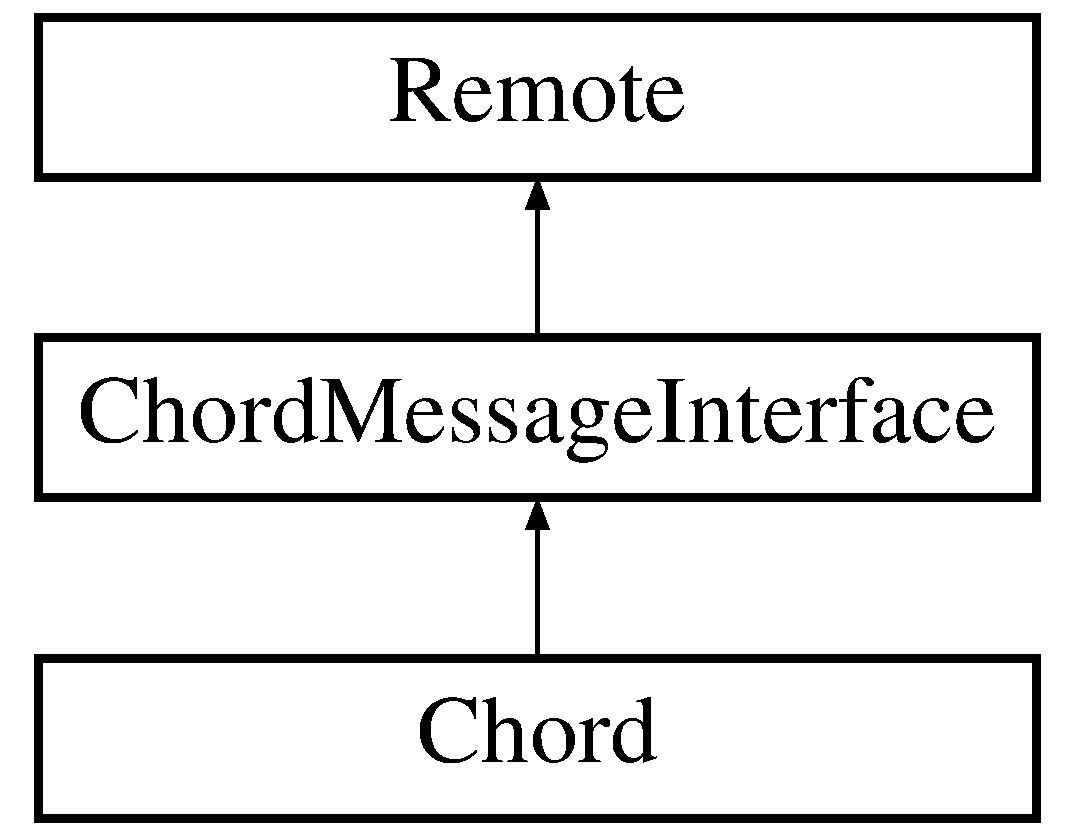
\includegraphics[height=3.000000cm]{interface_chord_message_interface}
\end{center}
\end{figure}
\subsection*{Public Member Functions}
\begin{DoxyCompactItemize}
\item 
\hyperlink{interface_chord_message_interface}{Chord\+Message\+Interface} \hyperlink{interface_chord_message_interface_ab07c08ba6088ef880eaf4ebae8281c51}{get\+Predecessor} ()  throws Remote\+Exception
\item 
\hyperlink{interface_chord_message_interface}{Chord\+Message\+Interface} \hyperlink{interface_chord_message_interface_a4e299d4b05537a4a07965dfe9f261fd0}{locate\+Successor} (int key)  throws Remote\+Exception
\item 
\hyperlink{interface_chord_message_interface}{Chord\+Message\+Interface} \hyperlink{interface_chord_message_interface_a7f47e9d5144a2af6904135bc05dfe8fd}{closest\+Preceding\+Node} (int key)  throws Remote\+Exception
\item 
void \hyperlink{interface_chord_message_interface_abc5a9483416a6b8ae7330b324869e236}{join\+Ring} (String Ip, int port)  throws Remote\+Exception
\item 
void \hyperlink{interface_chord_message_interface_a6afa0f7ae38d68a936a85216fe33d5ae}{leave\+Ring} ()  throws Remote\+Exception
\item 
void \hyperlink{interface_chord_message_interface_af6194ad846851fe7a8bd5f6bc8d36163}{set\+Successor} (\hyperlink{interface_chord_message_interface}{Chord\+Message\+Interface} p)  throws Remote\+Exception
\item 
void \hyperlink{interface_chord_message_interface_a28e2eda3267e1eaa8abec8adcf2604bb}{set\+Predeccesor} (\hyperlink{interface_chord_message_interface}{Chord\+Message\+Interface} s)  throws Remote\+Exception
\item 
void \hyperlink{interface_chord_message_interface_abbb77f94541073d79284d35f970e0eb4}{notify} (\hyperlink{interface_chord_message_interface}{Chord\+Message\+Interface} j)  throws Remote\+Exception
\item 
boolean \hyperlink{interface_chord_message_interface_a8165b3fb53905e657c70b66223197561}{is\+Alive} ()  throws Remote\+Exception
\item 
int \hyperlink{interface_chord_message_interface_acead95d9a7196f05b656462ab78138eb}{get\+Id} ()  throws Remote\+Exception
\item 
void \hyperlink{interface_chord_message_interface_a59a01f2e913b6b2e4b60ba0b77c90eba}{put} (int guid, Input\+Stream file)  throws I\+O\+Exception, Remote\+Exception
\item 
Input\+Stream \hyperlink{interface_chord_message_interface_a4cdb461c48fe643f4fb5fa420d017eb3}{get} (int id)  throws I\+O\+Exception, Remote\+Exception
\item 
void \hyperlink{interface_chord_message_interface_ab4d46beae8cea347c827b5618ea16104}{delete} (int id)  throws I\+O\+Exception, Remote\+Exception
\end{DoxyCompactItemize}


\subsection{Member Function Documentation}
\hypertarget{interface_chord_message_interface_a7f47e9d5144a2af6904135bc05dfe8fd}{}\label{interface_chord_message_interface_a7f47e9d5144a2af6904135bc05dfe8fd} 
\index{Chord\+Message\+Interface@{Chord\+Message\+Interface}!closest\+Preceding\+Node@{closest\+Preceding\+Node}}
\index{closest\+Preceding\+Node@{closest\+Preceding\+Node}!Chord\+Message\+Interface@{Chord\+Message\+Interface}}
\subsubsection{\texorpdfstring{closest\+Preceding\+Node()}{closestPrecedingNode()}}
{\footnotesize\ttfamily \hyperlink{interface_chord_message_interface}{Chord\+Message\+Interface} Chord\+Message\+Interface.\+closest\+Preceding\+Node (\begin{DoxyParamCaption}\item[{int}]{key }\end{DoxyParamCaption}) throws Remote\+Exception}



Implemented in \hyperlink{class_chord_a77a9443c945cf5482f59edf685c1dc70}{Chord}.

\hypertarget{interface_chord_message_interface_ab4d46beae8cea347c827b5618ea16104}{}\label{interface_chord_message_interface_ab4d46beae8cea347c827b5618ea16104} 
\index{Chord\+Message\+Interface@{Chord\+Message\+Interface}!delete@{delete}}
\index{delete@{delete}!Chord\+Message\+Interface@{Chord\+Message\+Interface}}
\subsubsection{\texorpdfstring{delete()}{delete()}}
{\footnotesize\ttfamily void Chord\+Message\+Interface.\+delete (\begin{DoxyParamCaption}\item[{int}]{id }\end{DoxyParamCaption}) throws I\+O\+Exception, Remote\+Exception}



Implemented in \hyperlink{class_chord_a83d9245c283baf440dc847cee154c8c6}{Chord}.

\hypertarget{interface_chord_message_interface_a4cdb461c48fe643f4fb5fa420d017eb3}{}\label{interface_chord_message_interface_a4cdb461c48fe643f4fb5fa420d017eb3} 
\index{Chord\+Message\+Interface@{Chord\+Message\+Interface}!get@{get}}
\index{get@{get}!Chord\+Message\+Interface@{Chord\+Message\+Interface}}
\subsubsection{\texorpdfstring{get()}{get()}}
{\footnotesize\ttfamily Input\+Stream Chord\+Message\+Interface.\+get (\begin{DoxyParamCaption}\item[{int}]{id }\end{DoxyParamCaption}) throws I\+O\+Exception, Remote\+Exception}



Implemented in \hyperlink{class_chord_a0425685114bc996226e87f417221c213}{Chord}.

\hypertarget{interface_chord_message_interface_acead95d9a7196f05b656462ab78138eb}{}\label{interface_chord_message_interface_acead95d9a7196f05b656462ab78138eb} 
\index{Chord\+Message\+Interface@{Chord\+Message\+Interface}!get\+Id@{get\+Id}}
\index{get\+Id@{get\+Id}!Chord\+Message\+Interface@{Chord\+Message\+Interface}}
\subsubsection{\texorpdfstring{get\+Id()}{getId()}}
{\footnotesize\ttfamily int Chord\+Message\+Interface.\+get\+Id (\begin{DoxyParamCaption}{ }\end{DoxyParamCaption}) throws Remote\+Exception}



Implemented in \hyperlink{class_chord_a7c6a50aff653bafc040f923c93061bdb}{Chord}.

\hypertarget{interface_chord_message_interface_ab07c08ba6088ef880eaf4ebae8281c51}{}\label{interface_chord_message_interface_ab07c08ba6088ef880eaf4ebae8281c51} 
\index{Chord\+Message\+Interface@{Chord\+Message\+Interface}!get\+Predecessor@{get\+Predecessor}}
\index{get\+Predecessor@{get\+Predecessor}!Chord\+Message\+Interface@{Chord\+Message\+Interface}}
\subsubsection{\texorpdfstring{get\+Predecessor()}{getPredecessor()}}
{\footnotesize\ttfamily \hyperlink{interface_chord_message_interface}{Chord\+Message\+Interface} Chord\+Message\+Interface.\+get\+Predecessor (\begin{DoxyParamCaption}{ }\end{DoxyParamCaption}) throws Remote\+Exception}



Implemented in \hyperlink{class_chord_a3f1aadce3820e808c80662bb61a58e34}{Chord}.

\hypertarget{interface_chord_message_interface_a8165b3fb53905e657c70b66223197561}{}\label{interface_chord_message_interface_a8165b3fb53905e657c70b66223197561} 
\index{Chord\+Message\+Interface@{Chord\+Message\+Interface}!is\+Alive@{is\+Alive}}
\index{is\+Alive@{is\+Alive}!Chord\+Message\+Interface@{Chord\+Message\+Interface}}
\subsubsection{\texorpdfstring{is\+Alive()}{isAlive()}}
{\footnotesize\ttfamily boolean Chord\+Message\+Interface.\+is\+Alive (\begin{DoxyParamCaption}{ }\end{DoxyParamCaption}) throws Remote\+Exception}



Implemented in \hyperlink{class_chord_a0a677ced19cc0cb5afd2a695977aeb95}{Chord}.

\hypertarget{interface_chord_message_interface_abc5a9483416a6b8ae7330b324869e236}{}\label{interface_chord_message_interface_abc5a9483416a6b8ae7330b324869e236} 
\index{Chord\+Message\+Interface@{Chord\+Message\+Interface}!join\+Ring@{join\+Ring}}
\index{join\+Ring@{join\+Ring}!Chord\+Message\+Interface@{Chord\+Message\+Interface}}
\subsubsection{\texorpdfstring{join\+Ring()}{joinRing()}}
{\footnotesize\ttfamily void Chord\+Message\+Interface.\+join\+Ring (\begin{DoxyParamCaption}\item[{String}]{Ip,  }\item[{int}]{port }\end{DoxyParamCaption}) throws Remote\+Exception}



Implemented in \hyperlink{class_chord_ace0b8d2768590d7527af155c6573cae7}{Chord}.

\hypertarget{interface_chord_message_interface_a6afa0f7ae38d68a936a85216fe33d5ae}{}\label{interface_chord_message_interface_a6afa0f7ae38d68a936a85216fe33d5ae} 
\index{Chord\+Message\+Interface@{Chord\+Message\+Interface}!leave\+Ring@{leave\+Ring}}
\index{leave\+Ring@{leave\+Ring}!Chord\+Message\+Interface@{Chord\+Message\+Interface}}
\subsubsection{\texorpdfstring{leave\+Ring()}{leaveRing()}}
{\footnotesize\ttfamily void Chord\+Message\+Interface.\+leave\+Ring (\begin{DoxyParamCaption}{ }\end{DoxyParamCaption}) throws Remote\+Exception}



Implemented in \hyperlink{class_chord_aa1906d1d721280b3a10a7754f604990a}{Chord}.

\hypertarget{interface_chord_message_interface_a4e299d4b05537a4a07965dfe9f261fd0}{}\label{interface_chord_message_interface_a4e299d4b05537a4a07965dfe9f261fd0} 
\index{Chord\+Message\+Interface@{Chord\+Message\+Interface}!locate\+Successor@{locate\+Successor}}
\index{locate\+Successor@{locate\+Successor}!Chord\+Message\+Interface@{Chord\+Message\+Interface}}
\subsubsection{\texorpdfstring{locate\+Successor()}{locateSuccessor()}}
{\footnotesize\ttfamily \hyperlink{interface_chord_message_interface}{Chord\+Message\+Interface} Chord\+Message\+Interface.\+locate\+Successor (\begin{DoxyParamCaption}\item[{int}]{key }\end{DoxyParamCaption}) throws Remote\+Exception}



Implemented in \hyperlink{class_chord_aa53f4f7c97122395a33d064460538db0}{Chord}.

\hypertarget{interface_chord_message_interface_abbb77f94541073d79284d35f970e0eb4}{}\label{interface_chord_message_interface_abbb77f94541073d79284d35f970e0eb4} 
\index{Chord\+Message\+Interface@{Chord\+Message\+Interface}!notify@{notify}}
\index{notify@{notify}!Chord\+Message\+Interface@{Chord\+Message\+Interface}}
\subsubsection{\texorpdfstring{notify()}{notify()}}
{\footnotesize\ttfamily void Chord\+Message\+Interface.\+notify (\begin{DoxyParamCaption}\item[{\hyperlink{interface_chord_message_interface}{Chord\+Message\+Interface}}]{j }\end{DoxyParamCaption}) throws Remote\+Exception}



Implemented in \hyperlink{class_chord_a4de8b8464782dd96d88deeb35b2f27a2}{Chord}.

\hypertarget{interface_chord_message_interface_a59a01f2e913b6b2e4b60ba0b77c90eba}{}\label{interface_chord_message_interface_a59a01f2e913b6b2e4b60ba0b77c90eba} 
\index{Chord\+Message\+Interface@{Chord\+Message\+Interface}!put@{put}}
\index{put@{put}!Chord\+Message\+Interface@{Chord\+Message\+Interface}}
\subsubsection{\texorpdfstring{put()}{put()}}
{\footnotesize\ttfamily void Chord\+Message\+Interface.\+put (\begin{DoxyParamCaption}\item[{int}]{guid,  }\item[{Input\+Stream}]{file }\end{DoxyParamCaption}) throws I\+O\+Exception, Remote\+Exception}



Implemented in \hyperlink{class_chord_a88829ad2bea7d036256fd55dab5945fd}{Chord}.

\hypertarget{interface_chord_message_interface_a28e2eda3267e1eaa8abec8adcf2604bb}{}\label{interface_chord_message_interface_a28e2eda3267e1eaa8abec8adcf2604bb} 
\index{Chord\+Message\+Interface@{Chord\+Message\+Interface}!set\+Predeccesor@{set\+Predeccesor}}
\index{set\+Predeccesor@{set\+Predeccesor}!Chord\+Message\+Interface@{Chord\+Message\+Interface}}
\subsubsection{\texorpdfstring{set\+Predeccesor()}{setPredeccesor()}}
{\footnotesize\ttfamily void Chord\+Message\+Interface.\+set\+Predeccesor (\begin{DoxyParamCaption}\item[{\hyperlink{interface_chord_message_interface}{Chord\+Message\+Interface}}]{s }\end{DoxyParamCaption}) throws Remote\+Exception}



Implemented in \hyperlink{class_chord_a03cd68070e7cf5a96e015773df7ab034}{Chord}.

\hypertarget{interface_chord_message_interface_af6194ad846851fe7a8bd5f6bc8d36163}{}\label{interface_chord_message_interface_af6194ad846851fe7a8bd5f6bc8d36163} 
\index{Chord\+Message\+Interface@{Chord\+Message\+Interface}!set\+Successor@{set\+Successor}}
\index{set\+Successor@{set\+Successor}!Chord\+Message\+Interface@{Chord\+Message\+Interface}}
\subsubsection{\texorpdfstring{set\+Successor()}{setSuccessor()}}
{\footnotesize\ttfamily void Chord\+Message\+Interface.\+set\+Successor (\begin{DoxyParamCaption}\item[{\hyperlink{interface_chord_message_interface}{Chord\+Message\+Interface}}]{p }\end{DoxyParamCaption}) throws Remote\+Exception}



Implemented in \hyperlink{class_chord_a7de61846981d5fd1b7a9b8a6c653dc76}{Chord}.



The documentation for this interface was generated from the following file\+:\begin{DoxyCompactItemize}
\item 
\hyperlink{_chord_message_interface_8java}{Chord\+Message\+Interface.\+java}\end{DoxyCompactItemize}

\hypertarget{class_chord_user}{}\section{Chord\+User Class Reference}
\label{class_chord_user}\index{Chord\+User@{Chord\+User}}
\subsection*{Public Member Functions}
\begin{DoxyCompactItemize}
\item 
\hyperlink{class_chord_user_ae885d3267350f3834158e42344854750}{Chord\+User} (int p)
\end{DoxyCompactItemize}
\subsection*{Static Public Member Functions}
\begin{DoxyCompactItemize}
\item 
static void \hyperlink{class_chord_user_a737455bbcfdae9ff4427063d77fb9038}{main} (String args\mbox{[}$\,$\mbox{]})
\end{DoxyCompactItemize}


\subsection{Constructor \& Destructor Documentation}
\hypertarget{class_chord_user_ae885d3267350f3834158e42344854750}{}\label{class_chord_user_ae885d3267350f3834158e42344854750} 
\index{Chord\+User@{Chord\+User}!Chord\+User@{Chord\+User}}
\index{Chord\+User@{Chord\+User}!Chord\+User@{Chord\+User}}
\subsubsection{\texorpdfstring{Chord\+User()}{ChordUser()}}
{\footnotesize\ttfamily Chord\+User.\+Chord\+User (\begin{DoxyParamCaption}\item[{int}]{p }\end{DoxyParamCaption})}

Begins the Process of joining writting reading deleting printing and leaving 

\subsection{Member Function Documentation}
\hypertarget{class_chord_user_a737455bbcfdae9ff4427063d77fb9038}{}\label{class_chord_user_a737455bbcfdae9ff4427063d77fb9038} 
\index{Chord\+User@{Chord\+User}!main@{main}}
\index{main@{main}!Chord\+User@{Chord\+User}}
\subsubsection{\texorpdfstring{main()}{main()}}
{\footnotesize\ttfamily static void Chord\+User.\+main (\begin{DoxyParamCaption}\item[{String}]{args\mbox{[}$\,$\mbox{]} }\end{DoxyParamCaption})\hspace{0.3cm}{\ttfamily [static]}}



The documentation for this class was generated from the following file\+:\begin{DoxyCompactItemize}
\item 
\hyperlink{_chord_user_8java}{Chord\+User.\+java}\end{DoxyCompactItemize}

\hypertarget{class_file_stream}{}\section{File\+Stream Class Reference}
\label{class_file_stream}\index{File\+Stream@{File\+Stream}}
Inheritance diagram for File\+Stream\+:\begin{figure}[H]
\begin{center}
\leavevmode
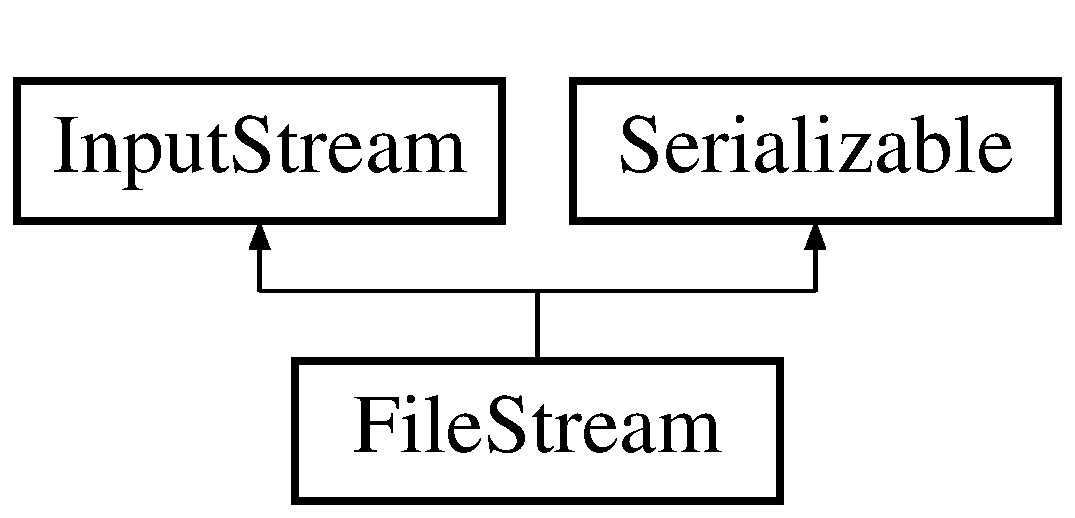
\includegraphics[height=2.000000cm]{class_file_stream}
\end{center}
\end{figure}
\subsection*{Public Member Functions}
\begin{DoxyCompactItemize}
\item 
\hyperlink{class_file_stream_a120b1fd6e4c74e93199d063da1c65b98}{File\+Stream} (String path\+Name)  throws File\+Not\+Found\+Exception, I\+O\+Exception    
\begin{DoxyCompactList}\small\item\em Constructor for \hyperlink{class_file_stream}{File\+Stream} that reads the file based on the parameter given. \end{DoxyCompactList}\item 
\hyperlink{class_file_stream_aa919eed4082491d09520911563d44efd}{File\+Stream} ()  throws File\+Not\+Found\+Exception    
\begin{DoxyCompactList}\small\item\em Default Constructor for \hyperlink{class_file_stream}{File\+Stream}. \end{DoxyCompactList}\item 
int \hyperlink{class_file_stream_a7f2ea40eff2241931a4ca971364cd532}{read} ()  throws I\+O\+Exception     
\begin{DoxyCompactList}\small\item\em Reads the file if the current position is less than the size. \end{DoxyCompactList}\item 
int \hyperlink{class_file_stream_a7dd240b96afa9e37f9a6bd8e4b99e48b}{available} ()  throws I\+O\+Exception     
\begin{DoxyCompactList}\small\item\em Checks that the current position has not exceeded the size of the file. \end{DoxyCompactList}\end{DoxyCompactItemize}
\subsection*{Private Attributes}
\begin{DoxyCompactItemize}
\item 
int \hyperlink{class_file_stream_a3d1da0e929f30d4ec245b2864285ad67}{current\+Position}
\item 
byte \mbox{[}$\,$\mbox{]} \hyperlink{class_file_stream_a3fd85491eb1625e6cd8414c19ee0defa}{byte\+Buffer}
\item 
int \hyperlink{class_file_stream_a0c4c084f04036a1a234eb04bf052bc1c}{size}
\end{DoxyCompactItemize}


\subsection{Constructor \& Destructor Documentation}
\hypertarget{class_file_stream_a120b1fd6e4c74e93199d063da1c65b98}{}\label{class_file_stream_a120b1fd6e4c74e93199d063da1c65b98} 
\index{File\+Stream@{File\+Stream}!File\+Stream@{File\+Stream}}
\index{File\+Stream@{File\+Stream}!File\+Stream@{File\+Stream}}
\subsubsection{\texorpdfstring{File\+Stream()}{FileStream()}\hspace{0.1cm}{\footnotesize\ttfamily [1/2]}}
{\footnotesize\ttfamily File\+Stream.\+File\+Stream (\begin{DoxyParamCaption}\item[{String}]{path\+Name }\end{DoxyParamCaption}) throws File\+Not\+Found\+Exception, I\+O\+Exception}



Constructor for \hyperlink{class_file_stream}{File\+Stream} that reads the file based on the parameter given. 

\hypertarget{class_file_stream_aa919eed4082491d09520911563d44efd}{}\label{class_file_stream_aa919eed4082491d09520911563d44efd} 
\index{File\+Stream@{File\+Stream}!File\+Stream@{File\+Stream}}
\index{File\+Stream@{File\+Stream}!File\+Stream@{File\+Stream}}
\subsubsection{\texorpdfstring{File\+Stream()}{FileStream()}\hspace{0.1cm}{\footnotesize\ttfamily [2/2]}}
{\footnotesize\ttfamily File\+Stream.\+File\+Stream (\begin{DoxyParamCaption}{ }\end{DoxyParamCaption}) throws File\+Not\+Found\+Exception}



Default Constructor for \hyperlink{class_file_stream}{File\+Stream}. 



\subsection{Member Function Documentation}
\hypertarget{class_file_stream_a7dd240b96afa9e37f9a6bd8e4b99e48b}{}\label{class_file_stream_a7dd240b96afa9e37f9a6bd8e4b99e48b} 
\index{File\+Stream@{File\+Stream}!available@{available}}
\index{available@{available}!File\+Stream@{File\+Stream}}
\subsubsection{\texorpdfstring{available()}{available()}}
{\footnotesize\ttfamily int File\+Stream.\+available (\begin{DoxyParamCaption}{ }\end{DoxyParamCaption}) throws I\+O\+Exception}



Checks that the current position has not exceeded the size of the file. 

\hypertarget{class_file_stream_a7f2ea40eff2241931a4ca971364cd532}{}\label{class_file_stream_a7f2ea40eff2241931a4ca971364cd532} 
\index{File\+Stream@{File\+Stream}!read@{read}}
\index{read@{read}!File\+Stream@{File\+Stream}}
\subsubsection{\texorpdfstring{read()}{read()}}
{\footnotesize\ttfamily int File\+Stream.\+read (\begin{DoxyParamCaption}{ }\end{DoxyParamCaption}) throws I\+O\+Exception}



Reads the file if the current position is less than the size. 



\subsection{Member Data Documentation}
\hypertarget{class_file_stream_a3fd85491eb1625e6cd8414c19ee0defa}{}\label{class_file_stream_a3fd85491eb1625e6cd8414c19ee0defa} 
\index{File\+Stream@{File\+Stream}!byte\+Buffer@{byte\+Buffer}}
\index{byte\+Buffer@{byte\+Buffer}!File\+Stream@{File\+Stream}}
\subsubsection{\texorpdfstring{byte\+Buffer}{byteBuffer}}
{\footnotesize\ttfamily byte \mbox{[}$\,$\mbox{]} File\+Stream.\+byte\+Buffer\hspace{0.3cm}{\ttfamily [private]}}

\hypertarget{class_file_stream_a3d1da0e929f30d4ec245b2864285ad67}{}\label{class_file_stream_a3d1da0e929f30d4ec245b2864285ad67} 
\index{File\+Stream@{File\+Stream}!current\+Position@{current\+Position}}
\index{current\+Position@{current\+Position}!File\+Stream@{File\+Stream}}
\subsubsection{\texorpdfstring{current\+Position}{currentPosition}}
{\footnotesize\ttfamily int File\+Stream.\+current\+Position\hspace{0.3cm}{\ttfamily [private]}}

\hypertarget{class_file_stream_a0c4c084f04036a1a234eb04bf052bc1c}{}\label{class_file_stream_a0c4c084f04036a1a234eb04bf052bc1c} 
\index{File\+Stream@{File\+Stream}!size@{size}}
\index{size@{size}!File\+Stream@{File\+Stream}}
\subsubsection{\texorpdfstring{size}{size}}
{\footnotesize\ttfamily int File\+Stream.\+size\hspace{0.3cm}{\ttfamily [private]}}



The documentation for this class was generated from the following file\+:\begin{DoxyCompactItemize}
\item 
\hyperlink{_file_stream_8java}{File\+Stream.\+java}\end{DoxyCompactItemize}

\hypertarget{class_shutdown}{}\section{Shutdown Class Reference}
\label{class_shutdown}\index{Shutdown@{Shutdown}}
Inheritance diagram for Shutdown\+:\begin{figure}[H]
\begin{center}
\leavevmode
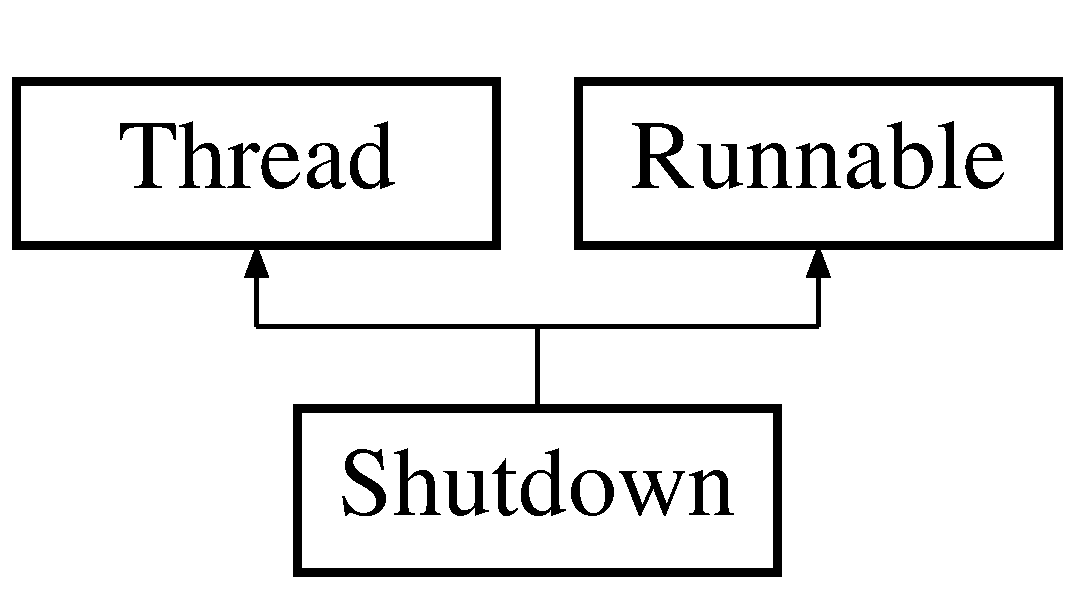
\includegraphics[height=2.000000cm]{class_shutdown}
\end{center}
\end{figure}
\subsection*{Public Member Functions}
\begin{DoxyCompactItemize}
\item 
\hyperlink{class_shutdown_a9753237b650b81387f45cb771f0da612}{Shutdown} (\hyperlink{interface_shutdown_interface}{Shutdown\+Interface} \hyperlink{class_shutdown_a8ed6d4f262656f4f6b5e30b8da025e0a}{shutdown})
\item 
void \hyperlink{class_shutdown_a5044221edbe8af603a9874518074b38d}{run} ()
\begin{DoxyCompactList}\small\item\em Catches the Control + C command. \end{DoxyCompactList}\end{DoxyCompactItemize}
\subsection*{Public Attributes}
\begin{DoxyCompactItemize}
\item 
\hyperlink{interface_shutdown_interface}{Shutdown\+Interface} \hyperlink{class_shutdown_a8ed6d4f262656f4f6b5e30b8da025e0a}{shutdown}
\end{DoxyCompactItemize}


\subsection{Constructor \& Destructor Documentation}
\hypertarget{class_shutdown_a9753237b650b81387f45cb771f0da612}{}\label{class_shutdown_a9753237b650b81387f45cb771f0da612} 
\index{Shutdown@{Shutdown}!Shutdown@{Shutdown}}
\index{Shutdown@{Shutdown}!Shutdown@{Shutdown}}
\subsubsection{\texorpdfstring{Shutdown()}{Shutdown()}}
{\footnotesize\ttfamily Shutdown.\+Shutdown (\begin{DoxyParamCaption}\item[{\hyperlink{interface_shutdown_interface}{Shutdown\+Interface}}]{shutdown }\end{DoxyParamCaption})}



\subsection{Member Function Documentation}
\hypertarget{class_shutdown_a5044221edbe8af603a9874518074b38d}{}\label{class_shutdown_a5044221edbe8af603a9874518074b38d} 
\index{Shutdown@{Shutdown}!run@{run}}
\index{run@{run}!Shutdown@{Shutdown}}
\subsubsection{\texorpdfstring{run()}{run()}}
{\footnotesize\ttfamily void Shutdown.\+run (\begin{DoxyParamCaption}{ }\end{DoxyParamCaption})}



Catches the Control + C command. 



\subsection{Member Data Documentation}
\hypertarget{class_shutdown_a8ed6d4f262656f4f6b5e30b8da025e0a}{}\label{class_shutdown_a8ed6d4f262656f4f6b5e30b8da025e0a} 
\index{Shutdown@{Shutdown}!shutdown@{shutdown}}
\index{shutdown@{shutdown}!Shutdown@{Shutdown}}
\subsubsection{\texorpdfstring{shutdown}{shutdown}}
{\footnotesize\ttfamily \hyperlink{interface_shutdown_interface}{Shutdown\+Interface} Shutdown.\+shutdown}



The documentation for this class was generated from the following file\+:\begin{DoxyCompactItemize}
\item 
\hyperlink{_shutdown_8java}{Shutdown.\+java}\end{DoxyCompactItemize}

\hypertarget{interface_shutdown_interface}{}\section{Shutdown\+Interface Interface Reference}
\label{interface_shutdown_interface}\index{Shutdown\+Interface@{Shutdown\+Interface}}
Inheritance diagram for Shutdown\+Interface\+:\begin{figure}[H]
\begin{center}
\leavevmode
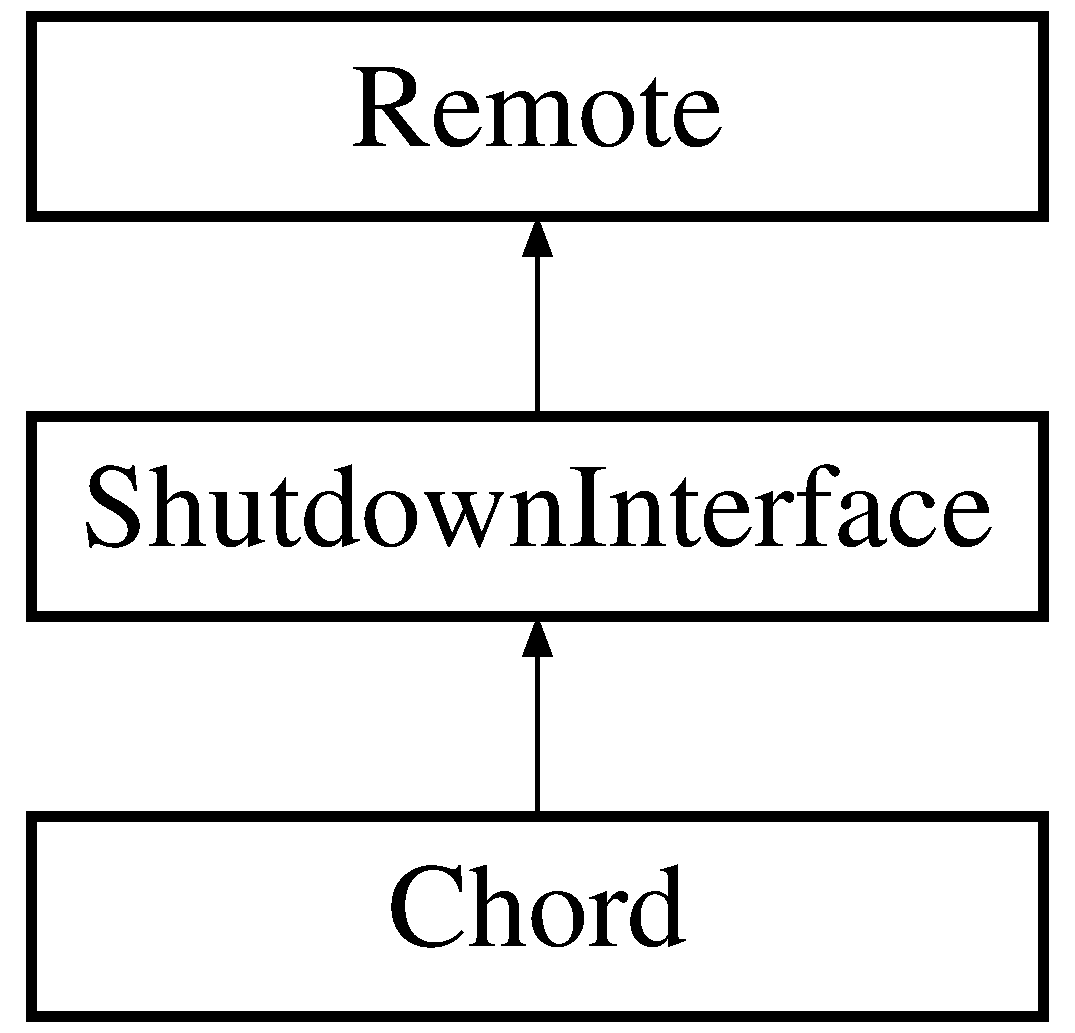
\includegraphics[height=3.000000cm]{interface_shutdown_interface}
\end{center}
\end{figure}
\subsection*{Public Member Functions}
\begin{DoxyCompactItemize}
\item 
void \hyperlink{interface_shutdown_interface_a16c9cfd61247e825a49564a4daab3286}{shutdown} ()  throws Remote\+Exception
\begin{DoxyCompactList}\small\item\em Catches the Control + C command. \end{DoxyCompactList}\end{DoxyCompactItemize}


\subsection{Member Function Documentation}
\hypertarget{interface_shutdown_interface_a16c9cfd61247e825a49564a4daab3286}{}\label{interface_shutdown_interface_a16c9cfd61247e825a49564a4daab3286} 
\index{Shutdown\+Interface@{Shutdown\+Interface}!shutdown@{shutdown}}
\index{shutdown@{shutdown}!Shutdown\+Interface@{Shutdown\+Interface}}
\subsubsection{\texorpdfstring{shutdown()}{shutdown()}}
{\footnotesize\ttfamily void Shutdown\+Interface.\+shutdown (\begin{DoxyParamCaption}{ }\end{DoxyParamCaption}) throws Remote\+Exception}



Catches the Control + C command. 



Implemented in \hyperlink{class_chord_a8616150947d5fa4095187325bc9f8a60}{Chord}.



The documentation for this interface was generated from the following file\+:\begin{DoxyCompactItemize}
\item 
\hyperlink{_shutdown_interface_8java}{Shutdown\+Interface.\+java}\end{DoxyCompactItemize}

\chapter{File Documentation}
\hypertarget{_chord_8java}{}\section{Chord.\+java File Reference}
\label{_chord_8java}\index{Chord.\+java@{Chord.\+java}}
\subsection*{Classes}
\begin{DoxyCompactItemize}
\item 
class \hyperlink{class_chord}{Chord}
\end{DoxyCompactItemize}

\hypertarget{_chord_message_interface_8java}{}\section{Chord\+Message\+Interface.\+java File Reference}
\label{_chord_message_interface_8java}\index{Chord\+Message\+Interface.\+java@{Chord\+Message\+Interface.\+java}}
\subsection*{Classes}
\begin{DoxyCompactItemize}
\item 
interface \hyperlink{interface_chord_message_interface}{Chord\+Message\+Interface}
\end{DoxyCompactItemize}

\hypertarget{_chord_user_8java}{}\section{Chord\+User.\+java File Reference}
\label{_chord_user_8java}\index{Chord\+User.\+java@{Chord\+User.\+java}}
\subsection*{Classes}
\begin{DoxyCompactItemize}
\item 
class \hyperlink{class_chord_user}{Chord\+User}
\end{DoxyCompactItemize}

\hypertarget{_file_stream_8java}{}\section{File\+Stream.\+java File Reference}
\label{_file_stream_8java}\index{File\+Stream.\+java@{File\+Stream.\+java}}
\subsection*{Classes}
\begin{DoxyCompactItemize}
\item 
class \hyperlink{class_file_stream}{File\+Stream}
\end{DoxyCompactItemize}

\hypertarget{_shutdown_8java}{}\section{Shutdown.\+java File Reference}
\label{_shutdown_8java}\index{Shutdown.\+java@{Shutdown.\+java}}
\subsection*{Classes}
\begin{DoxyCompactItemize}
\item 
class \hyperlink{class_shutdown}{Shutdown}
\end{DoxyCompactItemize}

\hypertarget{_shutdown_interface_8java}{}\section{Shutdown\+Interface.\+java File Reference}
\label{_shutdown_interface_8java}\index{Shutdown\+Interface.\+java@{Shutdown\+Interface.\+java}}
\subsection*{Classes}
\begin{DoxyCompactItemize}
\item 
interface \hyperlink{interface_shutdown_interface}{Shutdown\+Interface}
\end{DoxyCompactItemize}

%--- End generated contents ---

% Index
\backmatter
\newpage
\phantomsection
\clearemptydoublepage
\addcontentsline{toc}{chapter}{Index}
\printindex

\end{document}
